\documentclass[12pt, a4paper, oneside]{article}
\usepackage[left=3cm, right=2.5cm, top=2.5cm, bottom=2.5cm]{geometry}
\usepackage{times}
\usepackage[style=ieee]{biblatex}
\usepackage{tocloft, calc}
\usepackage{booktabs}
\usepackage{bbding} % marks

\usepackage{chngcntr} % table count reset
\usepackage{titlesec} % section title formatting

\usepackage{graphicx} % figure addition

\usepackage{setspace}

\usepackage{pgfgantt}

\usepackage{caption}

\usepackage{adjustbox}
\usepackage{array}

\usepackage{float}

% enumitem
\usepackage{enumitem}

% algorithms 
\usepackage[plain]{algorithm}
\usepackage{algorithmic}

\usepackage{amsmath}
\usepackage{amssymb}

\makeatletter
\renewcommand{\ALG@name}{Fig.}
\makeatother

\renewcommand{\figurename}{Fig.}

\onehalfspacing


\addbibresource{references.bib}

\let\indentorignal\cftsubsecindent

% table of content formatting fixes
\renewcommand{\contentsname}{\hfill \large{Table of Content}\hfill}
\renewcommand{\cftaftertoctitle}{\hfill}
\renewcommand{\cftaftertoctitleskip}{48pt}
\renewcommand{\cftdot}{} % dots in table of contents
\renewcommand{\cftsecpresnum}{CHAPTER\space}
\renewcommand{\cftsubsecindent}{12pt}
\addtocontents{toc}{\hfill\textbf{Title}\hfill\textbf{Page}\\[-12pt]\par}

% list of figures formatting fixes
\renewcommand{\listfigurename}{\hfill \large{List of figures}\hfill}
\renewcommand{\cftfigpresnum}{Fig.\space}
\renewcommand{\cftafterloftitleskip}{48pt}
\setlength{\cftfignumwidth}{\widthof{\textbf{Fig.~999~}\qquad}}
\addtocontents{lof}{\hspace{86pt}\textbf{Title}\hfill\textbf{Page}\\[-12pt]\par}

% list of tables formatting fixes
\renewcommand{\listtablename}{\hfill \large{List of table}\hfill}
\renewcommand{\cfttabpresnum}{Table\space}
\renewcommand{\cftafterlottitleskip}{48pt}
\setlength{\cfttabnumwidth}{\widthof{\textbf{Table~999~}\qquad}}
\addtocontents{lot}{\hspace{96pt}\textbf{Title}\hfill\textbf{Page}\\[-12pt]\par}

\counterwithin{table}{section}
\counterwithin{figure}{section}
\counterwithin{algorithm}{section}

% section title formatting [14pt]
\titleformat{\section}
{\large\bfseries}{\thesection}{1em}{}

% subsection title formatting [12pt, bold]
\titleformat{\subsection}
{\bfseries}{\thesubsection}{1em}{}

\begin{document}

\pagestyle{empty}
\begin{center}
    \Large{Report for the Degree of Master of Computer Science}\\[31pt]

    \LARGE{\textbf{DeepFake Face Detection using Dual Input CNN with Explainable AI (XAI)}}\\[93pt]


    \includegraphics*[width=1.6in,height=1.6in]{images/logo.png}\\[93pt]

    \Large{\textbf{Ujjwol Kayastha \\ (LC0003001469)}}\\[31pt]

    \Large{\textbf{
            Phoenix College of Management \\
            Computer Science and Multimedia Department \\
            Lincoln University, Malaysia
        }}\\[31pt]

    \Large{\textbf{
            July, 2024
        }}\\[31pt]
\end{center}

\pagestyle{empty}
\begin{center}
    \Large{Research Project for the Degree of master of Computer Science}\\[31pt]

    \LARGE{\textbf{DeepFake Face Detection using Dual Input CNN with Explainable AI (XAI)}}\\[93pt]

    \Large{\textbf{Supervised by Er. Santosh Dhungana, HOD, IT }}\\[31pt]

    \Large{A report submitted in partial fulfilment of the requirements for the degree of Master of Computer Science}\\[93pt]

    \Large{\textbf{Ujjwol Kayastha \\ (LC0003001469)}}\\[31pt]

    \Large{\textbf{
            Phoenix College of Management \\
            Computer Science and Multimedia Department \\
            Lincoln University, Malaysia
        }}\\[31pt]

    \Large{\textbf{
            July, 2024
        }}\\[31pt]
\end{center}

\pagenumbering{roman}

\pagestyle{plain}
\vspace*{52pt}
\begin{center}
    \large{\textbf{Declaration}}\\[31pt]
\end{center}

I hereby declare that this research project entitled \textbf{DeepFake Face Detection using  Dual Input CNN with Explainable AI (XAI)} is based on my original research work. Related works on the topic by other researchers have been duly acknowledged. I owe all the liabilities relating to accuracy and authenticity of the data and any other information included hereunder.

% 3 blank lines, 14pt, line spacing 1.5
\vspace{73pt}

\begin{flushleft}
    Signature \\
    Name of the Student: Ujjwol Kayastha \\
    Registration Number: LC0003001469 \\
    Date:
\end{flushleft}

\addtocontents{toc}{Declaration\hfill \thepage\par}

\pagestyle{plain}
\vspace*{52pt}
\begin{center}
    \large{\textbf{Recommendation}}\\[31pt]
\end{center}

This is to certify that this report entitled \textbf{DeepFake Face Detection using  Dual Input CNN with Explainable AI (XAI)} prepared
and submitted by \textbf{Ujjwol Kayastha}, in partial fulfilment of the requirements of the degree of Master of Computer Science (MCS) awarded by Lincoln University, has been completed under my supervision. I recommend the same for acceptance by Lincoln University.

% 3 blank lines, 14pt, line spacing 1.5
\vspace{73pt}

\begin{flushleft}
    Signature \\
    Er. Santosh Dhungana, HOD, IT\\
    Phoenix College of Management\\
    July, 2024
\end{flushleft}

\addtocontents{toc}{Recommendation\hfill \thepage\par}

\pagestyle{plain}
\vspace*{52pt}
\begin{center}
    \large{\textbf{Certificate}}\\[31pt]
\end{center}

The report entitled \textbf{DeepFake Face Detection using  Dual Input CNN with Explainable AI (XAI)} prepared and submitted by \textbf{Ujjwol Kayastha} has been examined by us and is accepted for the award of the degree of Master of Computer Science (MCS.) in Postgraduate by Lincoln University.


% 3 blank lines, 14pt, line spacing 1.5
\vspace{73pt}

\noindent
\textbf{Name of the external examiner in Bold} \hfill [Signature] \hfill [Date signed] \\
External examiner

\vspace{2cm}

\noindent
\textbf{Name of the report supervisor} \hfill [Signature] \hfill [Date signed] \\
Supervisor

\vspace{2cm}

\noindent
\textbf{Name of Head of Department or Principal} \hfill [Signature] \hfill [Date signed]

\addtocontents{toc}{Declaration\hfill \thepage\par}

\pagestyle{plain}
\vspace*{52pt}
\begin{center}
    \large{\textbf{Acknowledgements}}\\[31pt]
\end{center}
First of all, I would like to thank Lincoln University for giving me a chance to prepare the project in partial fulfilment of the requirements of the degree of Master of Computer Science (MCS) awarded by Lincoln University. 
After many months of hard work and sincere effort from my side, this research has been conducted. I would like to acknowledge the following notable personalities who have contributed their valuable efforts in different ways in creation of this research.

\par I would like to give special thanks to Mr. Santosh Dhungana, my research project supervisor for his professional guidance and valuable support and for his useful and constructive recommendations on this project.
I also owe deep gratitude to all reputed authors whose writings have provided me with the necessary guidance and invaluable materials for the enrichment of my research papers in all possible ways. 

\par My special appreciation goes to my colleague and to all my family members, teachers and friends for their continuous encouragement and help to complete this work directly or indirectly.
I wish to thank various people for their contribution to this project: Mr. Bibek Ale Magar and Mr. Dipesh Dulal for their valuable technical support on this project: Mr. Prakash Devkota for their help in collecting data necessary for the project .


% 3 blank lines, 14pt, line spacing 1.5
\vspace{73pt}

\begin{flushleft}
    Signature \\
    Name of the Student: Ujjwol Kayastha\\
    Registration Number: LC0003001469\\
    Date:
\end{flushleft}

\addtocontents{toc}{Acknowledgements\hfill \thepage\par}

\pagestyle{plain}
\vspace*{52pt}
\begin{center}
    \large{\textbf{Abstract}}\\[31pt]
\end{center}

Deepfakes represent a significant challenge in today's digital landscape, creating hyper-realistic fake images and videos using advanced AI techniques like Generative Adversarial Networks (GANs). This research aims to develop a robust model for detecting DeepFake images utilizing a Dual Input Convolutional Neural Network (DICNN) combined with Explainable AI (XAI) techniques. 
By employing LIME (Local Interpretable Model-agnostic Explanations) and opting for better optimizer RMSProp (Root Mean Square Propagation), this study enhances the interpretability and reliability of the detection process. 
The DICNN model achieved an impressive accuracy rate, demonstrating its efficacy in identifying deepfakes. 
This research contributes to the ongoing efforts to combat digital misinformation and underscores the importance of explainable AI in building trust and transparency in machine learning models.
In literature review, the research highlights the accuracy of DICNN with other state-of-the-art models and the significance of combining deep learning with explainable AI to ensure the reliability of AI systems.
This study also highlights the differences in accuracy between two optimizers, RMSProp and Adam. 


\begin{flushleft}
    \textbf{Keywords:} Deepfakes, Convolutional Neural Networks, Explainable AI, SHAP, LIME, Deep Learning, Face Images, Face Detection
\end{flushleft}

\begin{figure}[H]
    \centering
    
\includegraphics[height=6cm]{images/wordcloud.png}
    \label{fig:wordcloud}
 \end{figure}

\addtocontents{toc}{Abstract\hfill \thepage\par}

% section names in format Chapter: 1. Introduction
\tableofcontents
\addtocontents{toc}{Table of Content\hfill \thepage\par}
\cleardoublepage


\addtocontents{toc}{\protect\thispagestyle{empty}}

\listoffigures
\addtocontents{toc}{List of figures\hfill \thepage\par}
\cleardoublepage

\listoftables
\addtocontents{toc}{List of tables\hfill \thepage\par}
\cleardoublepage

\pagestyle{plain}
\pagenumbering{arabic}
\setcounter{page}{1}

\begin{section}[]{\uppercase{Introduction}}

    \addtocontents{toc}{\uppercase{Introduction}}

    \subsection{Background}
    In recent years, Artificial Intelligence (AI) and Machine Learning (ML) have rapid advancements which has led to development of Large Language Models (LLMs) like GPT-3, BERT, etc. 
    On the other hand, it has also led to proliferation of deepfake (DF) techniques. 
    Deepfake is a technique that uses AI to create fake images, videos, and audio recordings that appear real. 
    Deepfake technology has been used to create fake news, hoaxes, and other forms of misinformation. 
    It has been used to create fake images and videos of celebrities, politicians, and other public figures that can be used to blackmail, defame them or manipulate public opinion and influence elections.. 
    It can also be used to commit fraud or other forms of financial crimes, espionage or other forms of national security threats ot other forms of crimes or unethical behavior. \cite{Gaur2022}
    Advancement in Deep Learning models has enabled computer vision \cite{Guo2022}, Natural Language Processing (NLP) \cite{Shahi2021}, image processing \cite{Sitaula2022}, image steganography \cite{Bhandari2022} and smart transportation systems \cite{Gaur2022} to name a few.
    Photo editing softwares with inbuilt AI algorithms like Adobe Photoshop, GIMP, etc. have made it easier to create realistic and sophisticated deepfakes even to those who do not have photo editing experience. \cite{Wang2020}
    There are many easily available applications that can swap faces in videos and images like FaceApp, Zao, etc. that can be used to create deepfakes.
    When (General Adversarial Networks) GANs are used to create deepfakes, the researches done earlier that depended on deciphering the metadata of the images or videos to detect deepfakes are no longer effective along with splicing or copy-move detection techniques. Some of the researches are conducted to detect deepfakes produced by GANs. \cite{Li2022}
    NVIDIA has developed a deep learning model called StyleGAN2 that can generate high-quality deepfake images and videos that are almost indistinguishable from real images and videos which has made it possible for malicious actors to create deepfakes that can be used to deceive people and spread misinformation. \cite{Wong2022}
    We have been using biometric authentication systems like face recognition, fingerprint recognition, iris recognition, etc. on daily basis for financial transactions, unlocking smartphones, access management etc. \cite{Tran2017}
    Deepfake technology is evolving rapidly to create deepfakes that even makes us question the authenticity and integrity of information in digital world \Cites{Dang2020}{Rossler2019}.
    StyleGAN2 offers data-driven simulation relevant for deepfakes creation process optimization \cite{Zotov2022} which this research aims to explore.

    \par
    The ease of use and availability of deepfake technology has made it easier to generate hyper-realistic deepfakes. This has lessened the value of human integrity and dignity. Social media platforms like Facebook and Twitter (now X) have started to take steps to detect and remove deepfakes from their platforms. 
    Many cases of deepfakes have been reported: some of the notable incidents include the deepfake video of Barack Obama, Mark Zuckerberg, and Nancy Pelosi. In 2019, a United Kingdom-based energy company was scammed of 243,000 euros by a deepfake audio of the CEO's voice. \cite{Damiani2019}
    A report published back in 2020, more than 85,000 deepfake contents were which was doubled since initial observation in 2018. \cite{CyberNews2021}

    \subsubsection{Deepfake detection}
    The term “deepfake” is developed from the technology “deep learning,” a form of Artificial Intelligence (AI). Deep Learning (DL) and neural network technologies used to generate fake photos and
    videos that are difficult to distinguish from real ones are called “deepfake.” Deepfake detection is a challenging problem because deepfake images and videos are often very realistic and difficult to distinguish from real images and videos. 
    DF techniques are evolving rapidly and becoming more sophisticated, making it harder to detect deepfakes using traditional methods as it uses Deep Learning (DL) algorithms like Generative Adversarial Networks (GANs).
    Even though it can be used for good purposes like in the entertainment industry, it can also be used to create fake news, hoaxes, and other forms of misinformation or even security threats and privacy invasion.
    To maintain the trust and integrity of the digital world, it is important to develop effective deepfake detection techniques to detect and prevent its malicious usage. \cite{Korshunov2019}
    A plethora of researches have been conducted and published regarding deepfakes classification and detection using Machine Learning (ML) algorithms like Convolutional Neural Networks (CNNs), Recurrent Neural Networks (RNNs), Long Short-Term Memory (LSTM), etc. despite the fact that the technology is relatively new and evolving.

    \par Since the deepfake technology is evolving rapidly, it is important to develop deepfake detection models that can keep up with the evolving deepfake technology and mitigate the threat and impact of deepfakes. Not all algorithms are effective but some has shown promising results. Even though some ML algoriths perfoms well, it cannot be devoid of mistakes. The question arisis regarding trust, safety, accuracy and reliability. 
    European Union has proposed a regulation to regulate the use of deepfake technology to prevent its misuse and protect the privacy, security of individuals and right to explanation under General Data Protection Regulation (GDPR). \cite{Goodman2017}

    \subsubsection{Explainable AI (XAI)}
    ML algorithms are often considered as blackbox models as they are difficult to interpret and explain. This is where Explainable AI (XAI) comes into play. XAI is a set of techniques and methods that can be used to explain and interpret the decisions made by ML models. \cite{IBMExplainableAI}
    All of the mentioned work has achieved great accuracy, and DL algorithms have shown excellent
    performance. But because of the incomprehensible behavior of DL algorithms, there is a lack of liability
    and trust in the outcomes. Sometimes, this risk of making a wrong decision may outweigh the benefits of
    precision, speed, and decision-making efficacy. That is why XAI can help to understand and explain DL
    and neural networks better. Transparency of results and model improvement justify the adoption of XAI
    in the proposed method.
    This research uses XAI to showcase the image concentration of the sample images, which is novel in
    detecting deepfake images with high precision. The usage of XAI makes the proposed method very
    reliable for detecting deepfake.
    \par LIME \cite{Ribeiro2016} was one of the first two most significant efforts in the
    history of XAI. A tool called Lime may identify features from an image or text that are accountable for
    an ML model’s predictions. It is not model-specific. It can be applied to a large range of ML and DL
    algorithms. By feeding the comparable model inputs and watching how the predictions change, LIME
    tries to figure out the model’s most important features, or the major components that drive any given
    choice. This method provides easy explanations, such as whether the model’s predictions are driven by a
    specific word in a document or a feature in an image.

    \subsection{Statement of the problem}
    Deep Learning (DL) models like Convolutional Neural Networks (CNNs) have been used to detect deepfakes by analyzing the patterns and features in the images and videos to lessen the impact of deepfakes. \cite{Tolosana2020}
    However, the performance of the CNN models can be improved by using dual input CNN (DICNN) models that can take advantage of the dual input images to improve the detection accuracy of deepfakes. \cite{Bhandari2023}
    Despite advances in DeepFake detection, current methods face limitations in accuracy and interpretability. Traditional single input CNNs struggle with complex DeepFake patterns, and their decision-making processes remain opaque and lead to false negatives. There is a need for a more robust and explainable approach to detect and understand DeepFakes. Explainable AI (XAI) techniques aim to address the opacity issue by providing insights into how AI models make decisions. Furthermore, while dual input CNN models that can process multiple sources of information such as temporal and spatial features, have demonstrated improved performance.
    The proposed research aims to address these limitations by developing a dual input CNN model for DeepFake detection and enhancing its interpretability using XAI techniques and better optimizer.

    \subsection{Research questions}

    \begin{enumerate}[label=\bf{Q\arabic*}]
        \item How effective is a dual input CNN in detecting DeepFake faces compared to traditional single input CNN models with different optimizers?
        \item How can Explainable AI (XAI) techniques enhance the interpretability and reliability of DeepFake detection models?
    \end{enumerate}

    \subsection{Research objectives}
    The research aims to explore use of DICNN with XAI to develop DeepFake detection model by leveraging technologies. This research enhances the implementation of DICNN with XAI to improve the interpretability and reliability of DeepFake detection models with different datasets and advanced optimizer.
    The main objective of the proposed study is to anticipate and understand fraudulent images, and the major contributions are outlined in the points that follow:
    \begin{enumerate}[label=\bf{O\arabic*}]
        \item A dual branch CNN architecture is proposed to enlarge the view of the network with more prominent performance in auguring the fake faces.
        \item The study explores the blackbox approach of the DICNN model using SHAP to construct explanation-driven findings by utilizing shapely values.
    \end{enumerate}

    
    \subsection{Significance/rationale of the study}
    The growing challenges of deepfake technology have raised concerns about the authenticity and integrity of digital content. 
    The proposed research aims to develop a dual input CNN model for DeepFake detection and enhance its interpretability using XAI techniques. 
    The research will contribute to the development of more effective and reliable DeepFake detection models that can help mitigate the threat and impact of deepfakes and help improve the trust and integrity of the digital world. 
    The research will also help raise awareness about the importance of developing ethical AI and ML technologies that respect human rights and values. 
    The research will also help inspire future research and innovation in the field of AI and ML and contribute to the development of more advanced and reliable AI and ML technologies that can help address the challenges and opportunities of the digital age.

    \subsection{Limitation and scope of the study}
    \textbf{Limitations}
    \begin{enumerate}
        \item \textbf{Evolving Techniques}: Deepfake technology is rapidly evolving, and new methods may emerge that could potentially bypass the detection techniques developed in this study. Continuous updates and adaptations are necessary to keep the detection models effective.
        \item \textbf{Computational Resources}: The proposed dual input CNN and XAI techniques require substantial computational resources for training and evaluation, which may not be accessible to all researchers or practitioners.
        \item \textbf{Interpretability vs. Accuracy}: While Explainable AI aims to enhance the interpretability of the models, there may be a trade-off between achieving high accuracy and maintaining explainability, which needs careful consideration.
    \end{enumerate}

    \noindent\textbf{Scope}
    \begin{enumerate}
        \item \textbf{Dual Input CNN Model}: This study focuses on developing and evaluating a dual input CNN model that utilizes both spatial and temporal features for improved deepfake detection. The scope includes experimenting with different datasets and configurations to optimize performance.
        \item \textbf{Explainable AI Techniques}: The research integrates Explainable AI techniques, such as SHAP values, to interpret and explain the decision-making process of the CNN model. This will help in understanding how the model differentiates between real and fake content.
        \item \textbf{Comparative Analysis}: The study includes a comparative analysis of the proposed dual input's result generated with few datasets and different optimizers to evaluate the performance and interpretability of the model.
    \end{enumerate}

    \subsection{Ethical considerations}
    The research is conducted in accordance with ethical guidelines and principles to ensure the protection of human subjects and data privacy. Use of publicly available datasets and adherence to data protection regulations is done. Informed consent will be obtained for any data collection involving human subjects, and data anonymization techniques are used to protect privacy. The research also ensures transparency and accountability in reporting the results and interpretations to maintain the integrity and trustworthiness of the research findings. The references and citations are properly acknowledged to give credit to the original authors and sources. The research adheres to academic integrity and ethical standards in conducting and reporting the research.
    \par The research adheres to the ethical standards set forth by my academic institution and any relevant legal requirements, especially regarding data usage and privacy.



\end{section}

\pagebreak

\begin{section}[]{\uppercase{Literature Review}}
 \addtocontents{toc}{\uppercase{Literature Review}}

 Plethora of researches has been conducted to detect deepfakes using Deep Learning in various fields, especially in detection and recognition. From medical imaging, disease detections and classifications \cite{Khan2021} to sentiment analysis \cite{Alam2021}.
 Image recognition has created huge hype in field of DL. Many approaches like LSTM (Long Short-Term Memory), convolutional traces. Some have used GANs (Generative Adversarial Networks) for the deepfakes detection. \cite{Guarnera2020}
 Targeting specific features sets limitation as they can sometimes miss vital points.

 \subsection{Convolutional Neural Networks (CNNs)}
 The CNN (Convolutional Neural Networks) \cite{Saha2018} is powerful and efficient field in image classification and recognition. The DL algorithms takes image inputs and weights attributes and assign them to distinguish between real and deepfakse. Due to its less pre-processing and ability to learn characteristics, filters after training and its efficiency, many researches have been carried out.
 One of the researches \cite{Patel2020} proposes an idea to extract face from videos and classify as real or fake using various CNN methods, such as ResNet, Inception and VGG. Their most efficient architecture resulted 90.2\% validation accuracy.
 Researches has been carried out to develop system that can understand visual data which gave birth to Computer Vision. In 2012, AlexNet, an AI model, developed by researchers from University of Toronto, won ImageNet contest with 85\% accuracy that was driven by CNNs. \cite{AnalyticsVidhya2021}

    \begin{figure}[htbp]
        \centering
        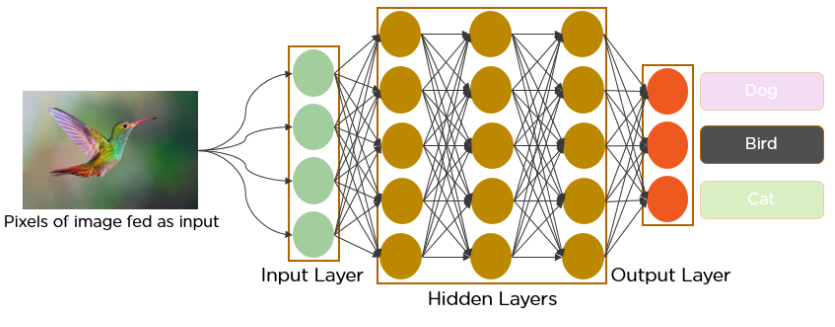
\includegraphics[width=\linewidth]{images/cnn.png}
        \caption{Simple representation of CNN}
        \label{fig:cnn}
    \end{figure}

CNNs are vital in computer vision tasks that includes object detection, image classification and segmentation. Modern CNNs uses Python to leverage advance techniques to extract and learn featurs from images. To train the models effectively, methos like hyperparameters, regularization and optimization techniques are crucial.


 \subsubsection{Single Input CNN Models}
 Deepfake detection on images, videos, or other form of media mostly uses traditional single input CNN that extract features from images using convolutional layers, pooling and fully connected layers for image classification.
 \begin{figure}[htbp]
    \centering
    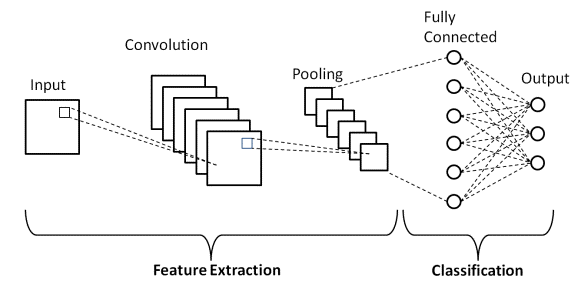
\includegraphics[width=\linewidth]{images/cnn-architecture.png}
    \caption{Single input CNN architecture}
    \label{fig:cnn-architecture}
\end{figure}

Fig. \ref{fig:cnn-architecture} depicts the main parts of CNN architecture that are stacked to generate output.


\subsubsection{Dual Input CNN Models}
DICNN (Dual Input Convolutional Neural Network) is based on base model of CNN. From numerous inputs it can update the parameters adaptively and identify deep patterns. 

\par In the base research paper \cite{Bhandari2023} referred, two input layers of size (224 x 224 x 3) were defined. The researcher processed one branch to continue with single convolution layer whose output was then flattened to concatenate flattened results of another branch. Two dense layers and dropout layers were added on top of that.
The integration of DICNN-XAI to augur fake face images and SHAP based explanation is depicted in the \ref*{fig:proposed-dicnn}. To explore blackbox approach of DICNN, after analysis it was fed to SHAP, an explainable AI.
\begin{figure}[htbp]
    \centering
    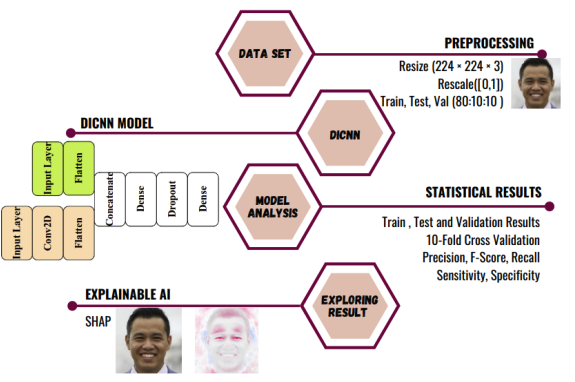
\includegraphics[width=\linewidth]{images/proposed-dicnn.png}
    \caption{Proposed DICNN model}
    \label{fig:proposed-dicnn}
\end{figure}

The model was developed in python using Keras and TensorFlow framework and the summary details for proposed DICNN architecture is depicted in 

 
% \begin{table}[htbp]
%     \centering
%     \begin{tabular}{>{\raggedright\arraybackslash}p{4cm} >{\raggedright\arraybackslash}p{4cm} r >{\raggedright\arraybackslash}p{3cm}}
%         \toprule
%         \textbf{Layer Name} & \textbf{Shape of Output} & \textbf{Param \#} & \textbf{Connected to} \\
%         \midrule
%         Input 1 & (None, 224, 224, 3) & 0 & - \\
%         Input 2 & (None, 224, 224, 3) & 0 & - \\
%         Conv2D & (None, 222, 222, 32) & 896 & Input 1 \\
%         Flatten 1 & (None, 150,528) & 0 & Input 2 \\
%         Flatten 2 & (None, 1,577,088) & 0 & Conv2D \\
%         Concatenate Layer & (None, 1,727,616) & 0 & [Flatten 1, Flatten 2] \\
%         Dense 1 & (None, 224) & 386,986,208 & Concatenate Layer \\
%         Dropout & (None, 224) & (None, 224) & Dense 1 \\
%         Dense 2 & (None, 2) & 450 & Dropout \\
%         \bottomrule
%     \end{tabular}
%     \caption{Summary details of proposed DICNN model}
%     \label{tab:proposed-dicnn-model}
% \end{table}

\vspace{2em}

Table reference:  \cite{Bhandari2023}
 \par \noindent Total params: 386,987,554 \\
 Trainable params: 386,987,554 \\
 Non-trainable params: 0

\subsection{Explainable AI (XAI)}
xai


\end{section}

\pagebreak
\begin{section}[]{\uppercase{Methodology}}
 \addtocontents{toc}{\uppercase{Methodology}}

 
\end{section}

\pagebreak

\begin{section}[]{\uppercase{Results and Discussion}}
 \addtocontents{toc}{\uppercase{Results and Discussion}}

 \subsection{Training Factors A}
 After augumentation of the data, the model was trained for 20 epochs with a train generator and validation generator, resulting in good model accuracy for each model. 
 The training factors have been summarized in the table \ref{tab:training_factors}.

 \begin{table}[htbp]
    \centering
    \begin{tabular}{ll}
        \toprule
        \textbf{Training factor} & \textbf{Values} \\
        \midrule
        Platform & Google Colaboratory \\
        TPU & Python 3 Google Compute Engine backend \\
        Optimizer & Adam \\
        Loss function & Categorical cross-entropy \\
        Learning rate & 0.001 \\
        Epoch & 20 \\
        Batch size & 10 \\
        \bottomrule
    \end{tabular}
    \caption{List of materials and tools used for training the model}
    \label{tab:training_factors}
\end{table}


\subsubsection{Training and Validation Results}

The table below presents the training and validation loss and accuracy metrics for each epoch during the training process of the dual-input Convolutional Neural Network (CNN) model. The training was conducted over 20 epochs. The performance metrics demonstrate the following key observations:

\begin{itemize}
    \item \textbf{Training Accuracy:} The training accuracy exhibits a high starting point at approximately 90.27\% in the first epoch, stabilizing around 85-90\% in subsequent epochs. This indicates the model's consistent learning pattern.
    \item \textbf{Validation Accuracy:} The validation accuracy is remarkably high, starting at 98.31\% in the first epoch and achieving a perfect accuracy of 100\% in the 18th epoch. The consistently high validation accuracy suggests that the model generalizes well to unseen data.
    \item \textbf{Training Loss:} The training loss shows fluctuations throughout the epochs, starting at 0.3247 and reaching 0.1859 by the 20th epoch. This variability could indicate the model's ongoing adjustments during the learning process.
    \item \textbf{Validation Loss:} The validation loss demonstrates significant variability, with values ranging from 0.0036 to 0.2476. The lowest validation loss occurs in the 18th epoch, at 0.0036, corresponding to the highest validation accuracy.
\end{itemize}

These results underscore the model's high performance and generalization capabilities. The low validation loss in several epochs highlights the model's effectiveness in minimizing error on unseen data, whereas the variability in training loss suggests continuous learning and optimization during training.

\begin{table}[htbp]
    \centering
    \begin{tabular}{llllll}
    \toprule
    \textbf{Epoch} & \textbf{Training Loss} & \textbf{Training Accuracy} & \textbf{Validation Loss} & \textbf{Validation Accuracy} \\ 
    \midrule
    1  & 0.3247 & 0.9027 & 0.0354 & 0.9831 \\ 
    \midrule
    2  & 0.2831 & 0.8749 & 0.0755 & 0.9746 \\ 
    \midrule
    3  & 0.3369 & 0.8315 & 0.2476 & 1.0000 \\ 
    \midrule
    4  & 0.3365 & 0.8627 & 0.0219 & 0.9915 \\ 
    \midrule
    5  & 0.2225 & 0.8766 & 0.2333 & 0.9153 \\ 
    \midrule
    6  & 0.3035 & 0.8401 & 0.0577 & 0.9661 \\ 
    \midrule
    7  & 0.2589 & 0.8532 & 0.0219 & 0.9915 \\ 
    \midrule
    8  & 0.2451 & 0.8636 & 0.0958 & 0.9492 \\ 
    \midrule
    9  & 0.1923 & 0.8871 & 0.0184 & 0.9915 \\ 
    \midrule
    10 & 0.2542 & 0.8566 & 0.0231 & 0.9831 \\ 
    \midrule
    11 & 0.2476 & 0.8610 & 0.0102 & 0.9915 \\ 
    \midrule
    12 & 0.2438 & 0.8471 & 0.0354 & 0.9831 \\ 
    \midrule
    13 & 0.2718 & 0.8514 & 0.1603 & 0.8898 \\ 
    \midrule
    14 & 0.2670 & 0.8332 & 0.0903 & 0.9576 \\ 
    \midrule
    15 & 0.2376 & 0.8784 & 0.0242 & 0.9831 \\ 
    \midrule
    16 & 0.2470 & 0.8566 & 0.0181 & 0.9915 \\ 
    \midrule
    17 & 0.1699 & 0.8454 & 0.0117 & 0.9915 \\ 
    \midrule
    18 & 0.1808 & 0.8766 & 0.0036 & 1.0000 \\ 
    \midrule
    19 & 0.2671 & 0.8714 & 0.0322 & 0.9915 \\ 
    \midrule
    20 & 0.1859 & 0.8940 & 0.0207 & 0.9915 \\ 
    \bottomrule
    \end{tabular}
    \caption{Epoch-wise Training and Validation Results for Adam Optimizer}
    \label{table:results-a}
    \end{table}
 
\begin{figure}[H]
    \centering
    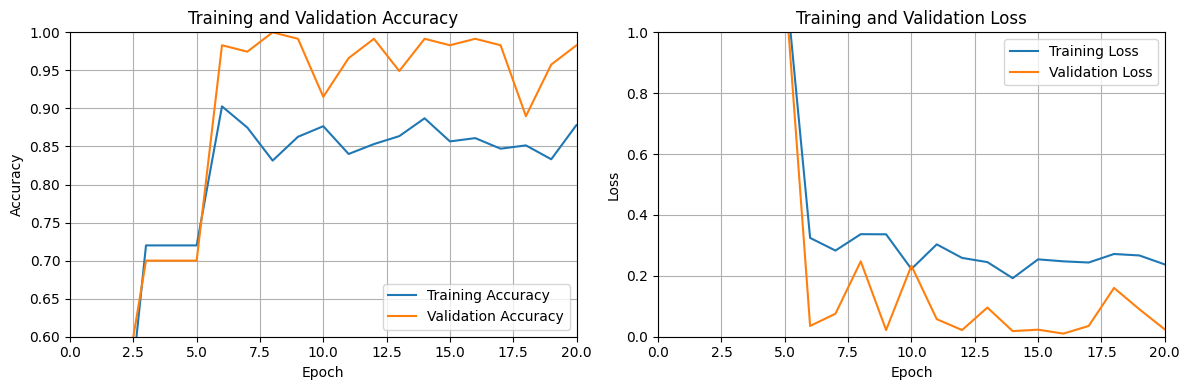
\includegraphics[width=\linewidth]{images/result.png}
    \caption{Training and Validation Results for Adam Optimizer}
    \label{fig:result}
\end{figure}

\subsection{Training Factors B}
The model was compiled with RMSProp optimizer and categorical cross-entropy loss function. RMSProp (Root Mean Square Propagation) is an optimization algorithm that uses the moving average of the squared gradient to normalize the gradient. It is an adaptive learning rate method that divides the learning rate by the moving average of the squared gradient. This helps to adjust the learning rate based on the gradient's magnitude, making it more stable and efficient.
The training factors have been summarized in the table \ref{tab:training_factors_b}.
\begin{table}[H]
    \centering
    \begin{tabular}{ll}
        \toprule
        \textbf{Training factor} & \textbf{Values} \\
        \midrule
        Platform & Google Colaboratory \\
        TPU & Python 3 Google Compute Engine backend \\
        Optimizer & RMSProp \\
        Loss function & Categorical cross-entropy \\
        Learning rate & 0.001 \\
        Epoch & 20 \\
        Batch size & 10 \\
        \bottomrule
    \end{tabular}
    \caption{List of materials and tools used for training the model}
    \label{tab:training_factors_b}
\end{table}



\subsubsection{Training and Validation Results}

The table below presents the training and validation loss and accuracy metrics for each epoch.
\begin{itemize}
    \item \textbf{Training Accuracy}: The training accuracy starts at approximately 77.76\% in the first epoch and shows a general upward trend, reaching 94.70\% by the 20th epoch. This indicates that the model is effectively learning and improving its performance.
    \item \textbf{Validation Accuracy}: The validation accuracy starts at a high 94.92\% in the first epoch, achieving perfect accuracy (100\%) in several epochs, including the second and final epochs. This suggests strong generalization ability to unseen data.
    \item \textbf{Training Loss}: The training loss starts high at 36.7045 in the first epoch but decreases significantly over the epochs, indicating the model's improved ability to minimize error during training.
    \item \textbf{Validation Loss}: The validation loss exhibits fluctuations, starting at 0.3475 in the first epoch, reaching as low as 0.0007 in the second epoch, and ending at 0.0063 in the final epoch. The low validation loss in multiple epochs highlights the model's effectiveness.
\end{itemize}

\begin{table}[H]
\centering
\begin{tabular}{llllll}
\toprule
\textbf{Epoch} & \textbf{Training Loss} & \textbf{Training Accuracy} & \textbf{Validation Loss} & \textbf{Validation Accuracy} \\ 
\midrule
    1  & 36.7045 & 0.7776 & 0.3475 & 0.9492 \\ 
    \midrule
    2  & 2.3207  & 0.8888 & 0.0007 & 1.0000 \\ 
    \midrule
    3  & 1.0619  & 0.9079 & 2.5053 & 0.8136 \\ 
    \midrule
    4  & 0.8817  & 0.9123 & 0.2394 & 0.9068 \\ 
    \midrule
    5  & 0.7055  & 0.9331 & 0.1060 & 0.9746 \\ 
    \midrule
    6  & 0.9905  & 0.9209 & 0.0614 & 0.9746 \\ 
    \midrule
    7  & 0.7818  & 0.9357 & 0.2718 & 0.9661 \\ 
    \midrule
    8  & 0.4616  & 0.9288 & 0.0055 & 1.0000 \\ 
    \midrule
    9  & 0.3379  & 0.9348 & 0.0353 & 0.9831 \\ 
    \midrule
    10 & 1.2596  & 0.8871 & 0.0474 & 0.9915 \\ 
    \midrule
    11 & 0.3767  & 0.9453 & 0.0691 & 0.9915 \\ 
    \midrule
    12 & 0.3609  & 0.9409 & 0.1279 & 0.9746 \\ 
    \midrule
    13 & 0.8072  & 0.9070 & 0.0652 & 0.9831 \\ 
    \midrule
    14 & 0.3556  & 0.9322 & 0.0606 & 0.9746 \\ 
    \midrule
    15 & 0.6149  & 0.9253 & 0.0292 & 0.9915 \\ 
    \midrule
    16 & 0.4864  & 0.9288 & 0.0336 & 0.9746 \\ 
    \midrule
    17 & 0.5084  & 0.9331 & 0.0493 & 0.9661 \\ 
    \midrule
    18 & 0.3350  & 0.9513 & 0.0325 & 0.9746 \\ 
    \midrule
    19 & 0.3296  & 0.9288 & 0.1307 & 0.9068 \\ 
    \midrule
    20 & 0.1756  & 0.9470 & 0.0063 & 1.0000 \\ 
\bottomrule
\end{tabular}
\caption{Epoch-wise Training and Validation Metrics for RMSProp Optimizer}
\label{table:results-b}
\end{table}

\begin{figure}[H]
    \centering
    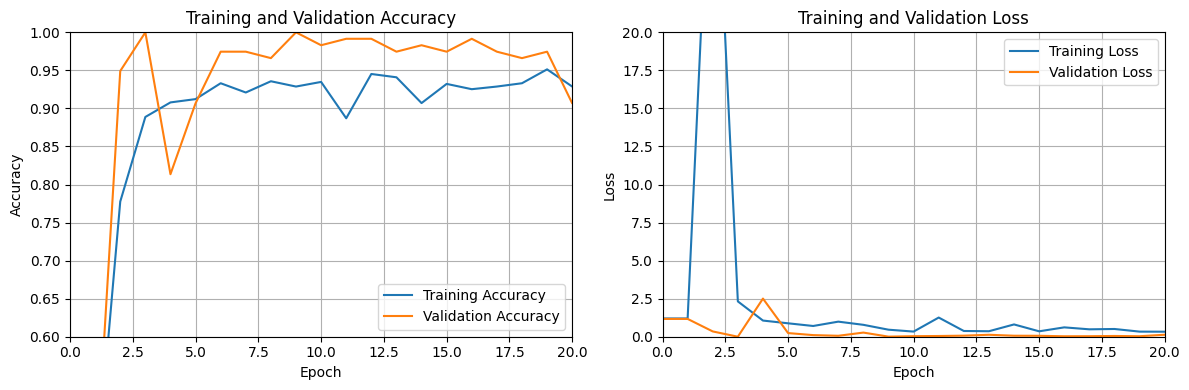
\includegraphics[width=\linewidth]{images/result-2.png}
    \caption{Training and Validation Results for RMSProp Optimizer}
    \label{fig:result-2}
\end{figure}

\subsection{Discussion}
\subsubsection{Performance Validation with XAI}
To analyze the deefake, it is crucial to identify real from fakes and that the model is not biased. SHAP was employed in the base paper, whereas LIME was added to the research to provide more explanation.
The Local Interpretable Model-Agnostic Explanations (LIME) algorithm was applied to the proposed
model. The LIME algorithm is a popular XAI algorithm that can be used to explain image samples with
visual representation. LIME is a model-agnostic algorithm that approximates the local linear behavior of the model.
LIME helps us understand why the model made a particular decision by showing which parts of the image were important.
The highlighted regions are crucial for the model's prediction. For a real image, these are the areas that convinced the model it is real. For a fake image, these are the areas that convinced the model it is fake.
This helps humans understand the model's decision-making process, making it more transparent and trustworthy.

%arrance lime-fake.png and lime-real.png in 2 columns
\begin{figure}[H]
    \centering
    \begin{minipage}{0.45\textwidth}
        \centering
        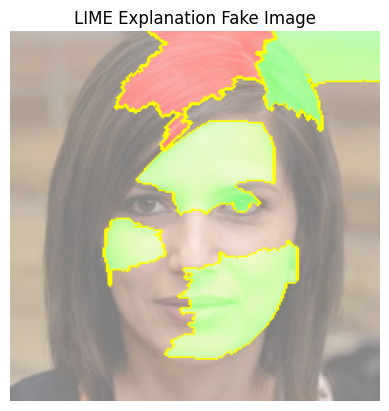
\includegraphics[width=\linewidth]{images/lime-fake.png}
        \captionsetup{font=small}
        \caption{LIME Explanation for Fake Image}
        \label{fig:lime-fake}
    \end{minipage}
    \hfill
    \begin{minipage}{0.45\textwidth}
        \centering
        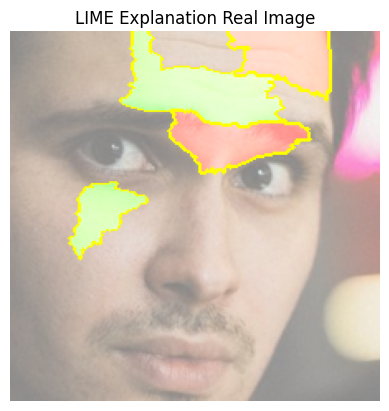
\includegraphics[width=\linewidth]{images/lime-real.png}
        \captionsetup{font=small}
        \caption{LIME Explanation for Real Image}
        \label{fig:lime-real}
    \end{minipage}
\end{figure}



\end{section}

\pagebreak

\begin{section}[]{\uppercase{Conclusion and Recommendation}}
 \addtocontents{toc}{\uppercase{Conclusion and Recommendation}}

 \subsection{Conclusion}
The main objective of the project are to detect deepfakes with the help of Dual Input Convolutional Neural Network (DICNN) and to evaluate the model. The research has been conducted to detect deepfakes using Deep Learning in various fields, especially in detection and recognition. 
The research will shed light on the use of and help in day-to-day life. 
The use of XAI in deepfake image detection is novel and is exclusively present in this research paper. The proposed system provides 99.17\% accuracy in detecting
deepfake images from real images. The results indicate that the proposed method is very robust at
detecting deepfake images and is also reliable and trustworthy because of the verification and integration
from XAI.
The SHAP \& LIME explainable AI are also used in this
research to describe which component of the image from the dataset caused the model to create specific
classifications, ensuring the model’s validity and reliability.
If this system was available in public, it would save hassle of dealing with fake content and fake information.
Eventhough, XAI is limited to images in present context, in near future, we can expect it to be used in videos and other forms of media.
Moreover, the research demonstrates the value of combining deep learning with explainable AI to ensure the transparency and trustworthiness of AI systems.



\subsection{Recommendation}
The trust in the developed model and its predictions are based on how well the model is trained and how well the model is explained. 
Further research can be carried out to improve the model and to make it more efficient and reliable. The findings show that the DICNN-XAI model is very efficient in detecting deepfake images from real images with high accuracy. This enhances the trust in DL systems enabling better understanding of system behavior.
In addition to SHAP used in base research paper, LIME was added to the research to provide more explanation to the model with 10x times the dataset. The results were compared and the model was evaluated. This study can be extended to videos and other forms of media to detect deepfakes. It can be used for other XAI algorithms like GradCAM, that can improve auguring problems.
Also more diverse data can be used to train the model to make it more robust and reliable. More heterogeneous data can ensure that the model developed is efficient. This current model can be extended to detect deepfakes in videos, which pose a more complex challenge due to the temporal dynamics involved.
 
\end{section}

\pagebreak



\newpage
\addcontentsline{toc}{section}{REFERENCES}
\printbibliography[title=REFERENCES]

\end{document}
